The following chapter is dedicated to giving the reader an overview of an $O(k^2 n \log n)$ 
time algorithm for solving the shortest path with obstacle violation problem. First we present an 
overview of the Hershberger-Suri algorithm, which solves the shortest path with no violation, 
in an optimal $O(n \log n)$ time \cite{HershbergerS99}. This algorithm produces a shortest 
path map, which divides the free space (free space being the plane minus the interior of the 
obstacles) into region where each subdivision will have the same shortest sub-path to 
all points in the area. This structure can then be extended for the purpose of calculating 
shortest paths with violation, which we will present an intuitive idea on how this is done. 
Finally we present an algorithm which will combine the Hershberger-Suri algorithm with a 
modified version of the same algorithm, to produce a shortest $k$-path map, a subdivision 
which has the shortest sub-path to all points in an area with $k$ violations, in time $O(k^2 
n \log n)$. This result is due to Hershberger, Kumar and Suri \cite{HershbergerKS17}.

\section{The Hershberger-Suri algorithm overview}

The Hershberger-Suri algorithm is an algorithm for computing the shortest 
path in a plane in the presence of obstacles without violations. The 
Hershberger-Suri algorithm was proven to be optimal-time in \cite{HershbergerS99}, 
with its $O(n \log n)$ running time, with $n$ being the total number of vertices 
of the obstacles located in the plane. This is done by computing a shortest path map 
which is  a map containing the shortest paths from a fixed source point $s$, to all 
other points in the plane. This is done by subdividing the plane into a finite number
of regions, where all the points in such a region have the same shortest sub-path
from $s$. This map can be constructed in $O(n\log n)$ time and requires $O(n\log n)$ 
space A query for a shortest path can be processed in $O(\log n)$
time.

The first step in the Hershberger-Suri algorithm is to use an implementation of
the continuous Dijkstra method, which purpose is to give a distance from the
source $s$ to each vertex and edge in the plane. The continuous Dijkstra method
is a theoretical tool to simulate a propagation of a unit speed wavefront in a
free space, where $s$ sends out the first emission, which propagates through
the plane and collides with obstacles. Upon collision between a wavefront and
a vertex in an obstacle, then this vertex will also start emitting a wavefront
of its own, with its weight equal to the time it took from $s$ started to emit
its wavefront until a contact (with any wavefront). 

Hershberger and Suri introduced two new ideas to speed the implementation of the
continuous Dijkstra method up compared to previous attempts, the first being a 
quad-tree-like subdivision of the plane, which we'll later introduce as a conforming 
subdivision, and the second being an approximate wavefront, which introduces a
bit of slack in the calculation of the collision-time of the wavefronts.

The first idea is grounded in the observation that a wavefront of the type in the 
continuous Dijkstra method, will be quite complicated to implement directly. 
A subdivision of the plane into well-behaved regions will be a way around this. 
This subdivision is constructed in such a way that it aids the propagation of the 
wavefronts. This is done by temporarily ignoring the line segments(edges) between the 
vertices in the obstacles, and subdividing the plane into a grid-like subdivision of 
size $O(n)$ around the vertices. Each cell in this subdivision, (the conforming 
subdivision) will only have a constant number of straight line edges, and will contain 
at most one obstacle vertex. This construction means that the subdivision satisfies the 
following crucial property: for any edge $e$ of the subdivision, there are $O(1)$ cells 
within distance $2|e|$ of $e$, which will be crucial in bounding the overall complexity
of the subdivision.

The obstacle line segments will then be inserted into the subdivision, while
maintaining both the linear size of the subdivision and its conforming property, except 
now a non-obstacle edge $e$ will have the property of having $O(1)$ cells within 
shortest path distance $2|e|$ of the edge.

These cells will then form the basis for the \textit{unitspeed} propagation in the 
algorithm, which will act as the wavefront propagation in the algorithm. This means 
that at each step the wavefront will propagated through one cell at a time for each 
time count. Since the descriptive complexity of each cell will be constant the 
algorithm will perform efficiently in the propagation through of the cells.

Inside each of these cells there will be two types of event: the first being a
collision between a wavefront and an obstacle, which is quite easy to handle. The 
second type of event will be a collisions between two wavefronts which will be more 
complex problem to handle. There will be two different types of collisions between two 
wavefronts, the first being the collisions where the wavelets are neighbors in the 
wavefront, and the second being collisions between non-neighboring wavelets. Here two 
wavefronts are waves emitted from two different sources, and two wavelets being two 
parts of the wave arch emitted from one source. The case of colliding neighboring 
wavelets occurs when a wavelet would be engulfed by the expansion of wavelets of its 
two neighbors and should be quite easy to detect and process. The collision between 
non-neighboring wavelets, however are more troublesome, and to process these we make 
use of the second idea: approximate wavefront.

The idea of approximating wavefronts is the abandonment of trying to compute the exact 
time of collision and instead maintaining two separate wavefronts approaching the edge 
from opposite sides. Each of these wavefronts is an \textit{approximate wavefront}, 
representing the wavefront that hits the edge from only one side. This leads to the 
other wavefronts which arrives at the edge after first wavefront, wont be recorded by 
the edge, due to it being slower than the initial arriving wavefront.

As mentioned above the Hershberger-Suri algorithm make use of timers to estimate the 
distance between two points in the plane but also to estimate when each edge in the 
subdivision would be engulfed by the wavefronts. A critical task of these timers is to 
ensure that the collision between two wavefronts which are used in the construction of 
the shortest path map, is measured in a small proximity of their actual collision, and 
therefore location.

At the end of the propagation phase, all the collision information is collected, and 
then a Voronoi diagram like technique is used in each cell to compute the collision 
events in that cell precisely. These collisions determines the edges of the final 
shortest path map, which will give us the shortest path to every point in the plane.

\section{From no violations to k-violations}

Previously, we've given an overview of the Hershberger-Suri algorithm which calculates a 
shortest path map ($SPM$) in $O(n\log n)$ time from a source point $s$ 
\cite{HershbergerS99}. By modifying the algorithm, and using it in as a subroutine 
Hershberger, Kumar and Suri showed an algorithm for calculating the shortest path map, 
where every route would violated at most $k$ obstacles from $s$ to an endpoint 
$t$\cite{HershbergerKS17}. This  is done by calculating a shortest $k$-path map, which in 
essence would produce a subdivision of the plane into regions, as done by the 
Hershberger-Suri algorithm, but with the guarantee of every path violating at most $k$ 
obstacles. A way to better understand how such a map would be calculated is by using the 
metaphor of a parking garage. Here every obstacle would be seen as an elevator from one 
floor $i$ to the next floor $i+1$. This would imply one could only take at most $k$ 
elevator trips when taking the path from $s$ to $t$. When thinking about the problem in 
this way, it seems quite natural to think of the construction of $SPM_k$ iteratively, 
starting by making the $SPM_0$ map, which is done by the Hershberger-Suri algorithm, and 
then from this construct the $SPM_1$ map, and for each iteration going one floor up, 
until we reach $SPM_{k-1}$.

\section{Construction of a shortest $k$-path map}

The $O(k^2 n \log n)$ implementation of shortest path with obstacle violation, makes use 
both of a unchanged and a modification version of the Hershberger-Suri algorithm. The 
unchanged version is used to prepare the $SPM_0$ map, which the modified version then 
uses to iteratively calculate the $SPM_k$ map. The change is due to the unchanged 
algorithm starts the wave propagation from a source point $s$ which propagates through 
the plane. 

\begin{figure}[H]
\centering
\caption{}
\begin{subfigure}{.5\textwidth}
  \centering 
  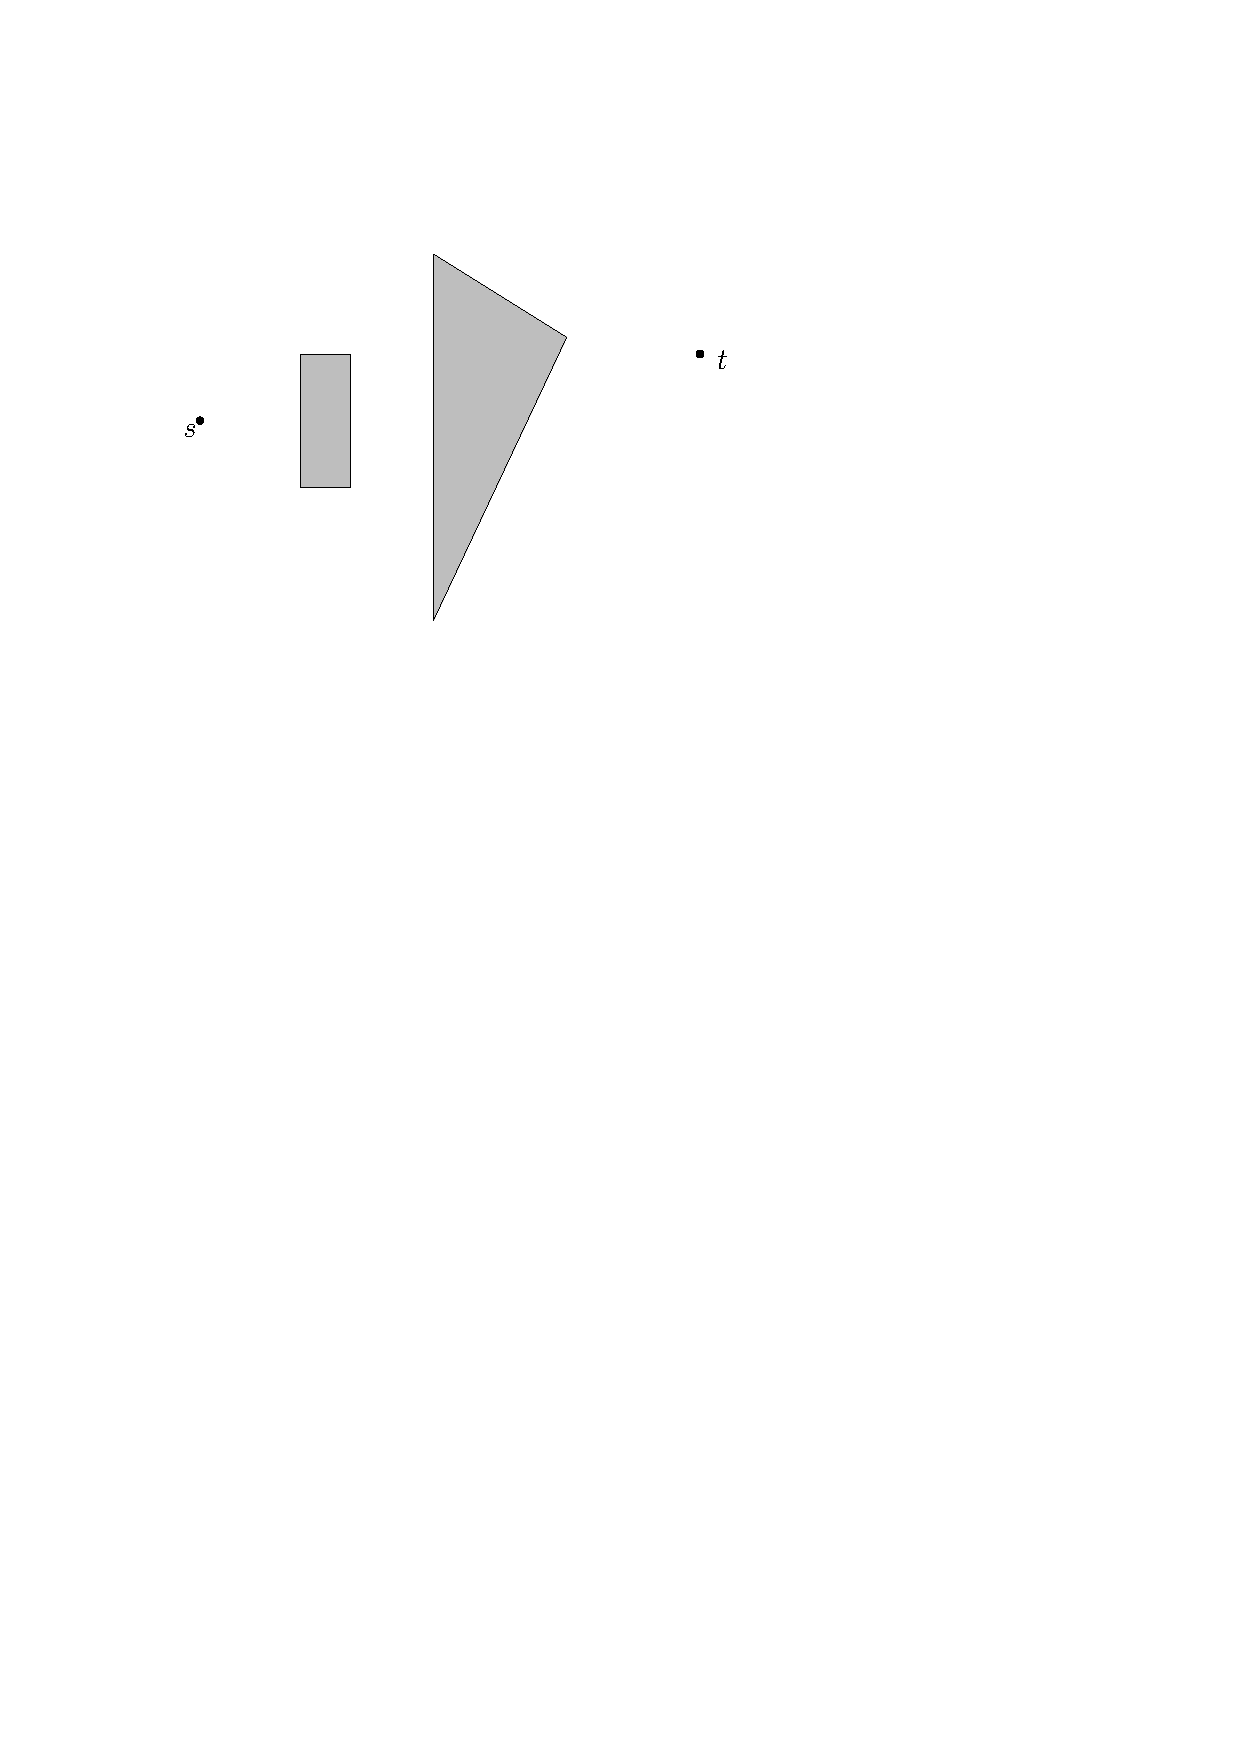
\includegraphics[width=.95\linewidth]{figures/prespm0.pdf}
  \caption{A plane with source $s$ and target $t$ with two obstacles}
  \label{fig:spmplane}
\end{subfigure}%
\begin{subfigure}{.5\textwidth}
  \centering
  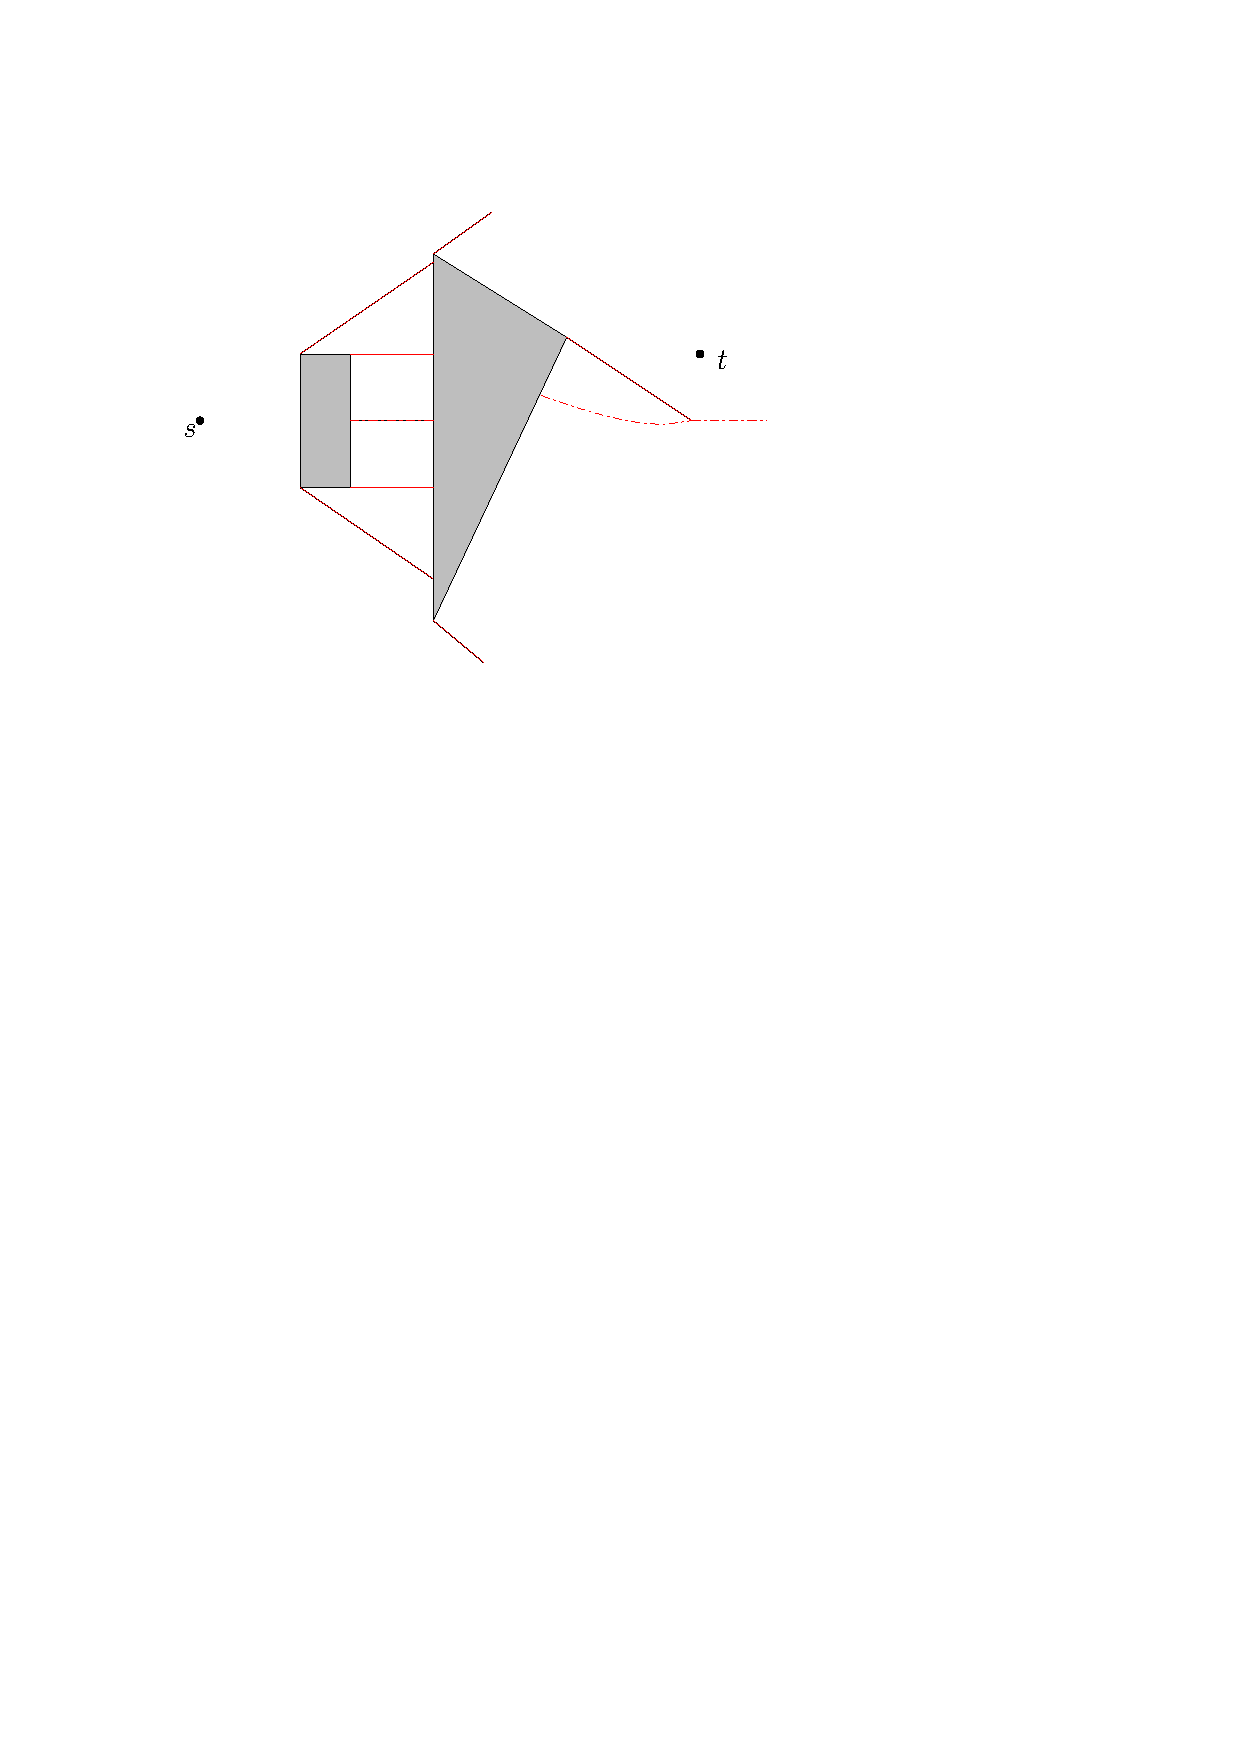
\includegraphics[width=.95\linewidth]{figures/spm0.pdf}
  \caption{A plane with the regions of $SPM_0$ drawn. The dash dotted line is the edge of two 
  		   areas where there is two shortest paths of equal length}
  \label{fig:planewithspm0drawn}
\end{subfigure}
\end{figure}

Above we see in figure \ref{fig:spmplane} a plane with $s$ and $t$ and two obstacles. Figure 
\ref{fig:planewithspm0drawn} shows a drawing of the $SPM_0$, which the unmodified 
Hershberger-Suri algorithm will calculate. 

\begin{figure}[H]
\caption{}
\centering
\begin{subfigure}{.5\textwidth}
  \centering
  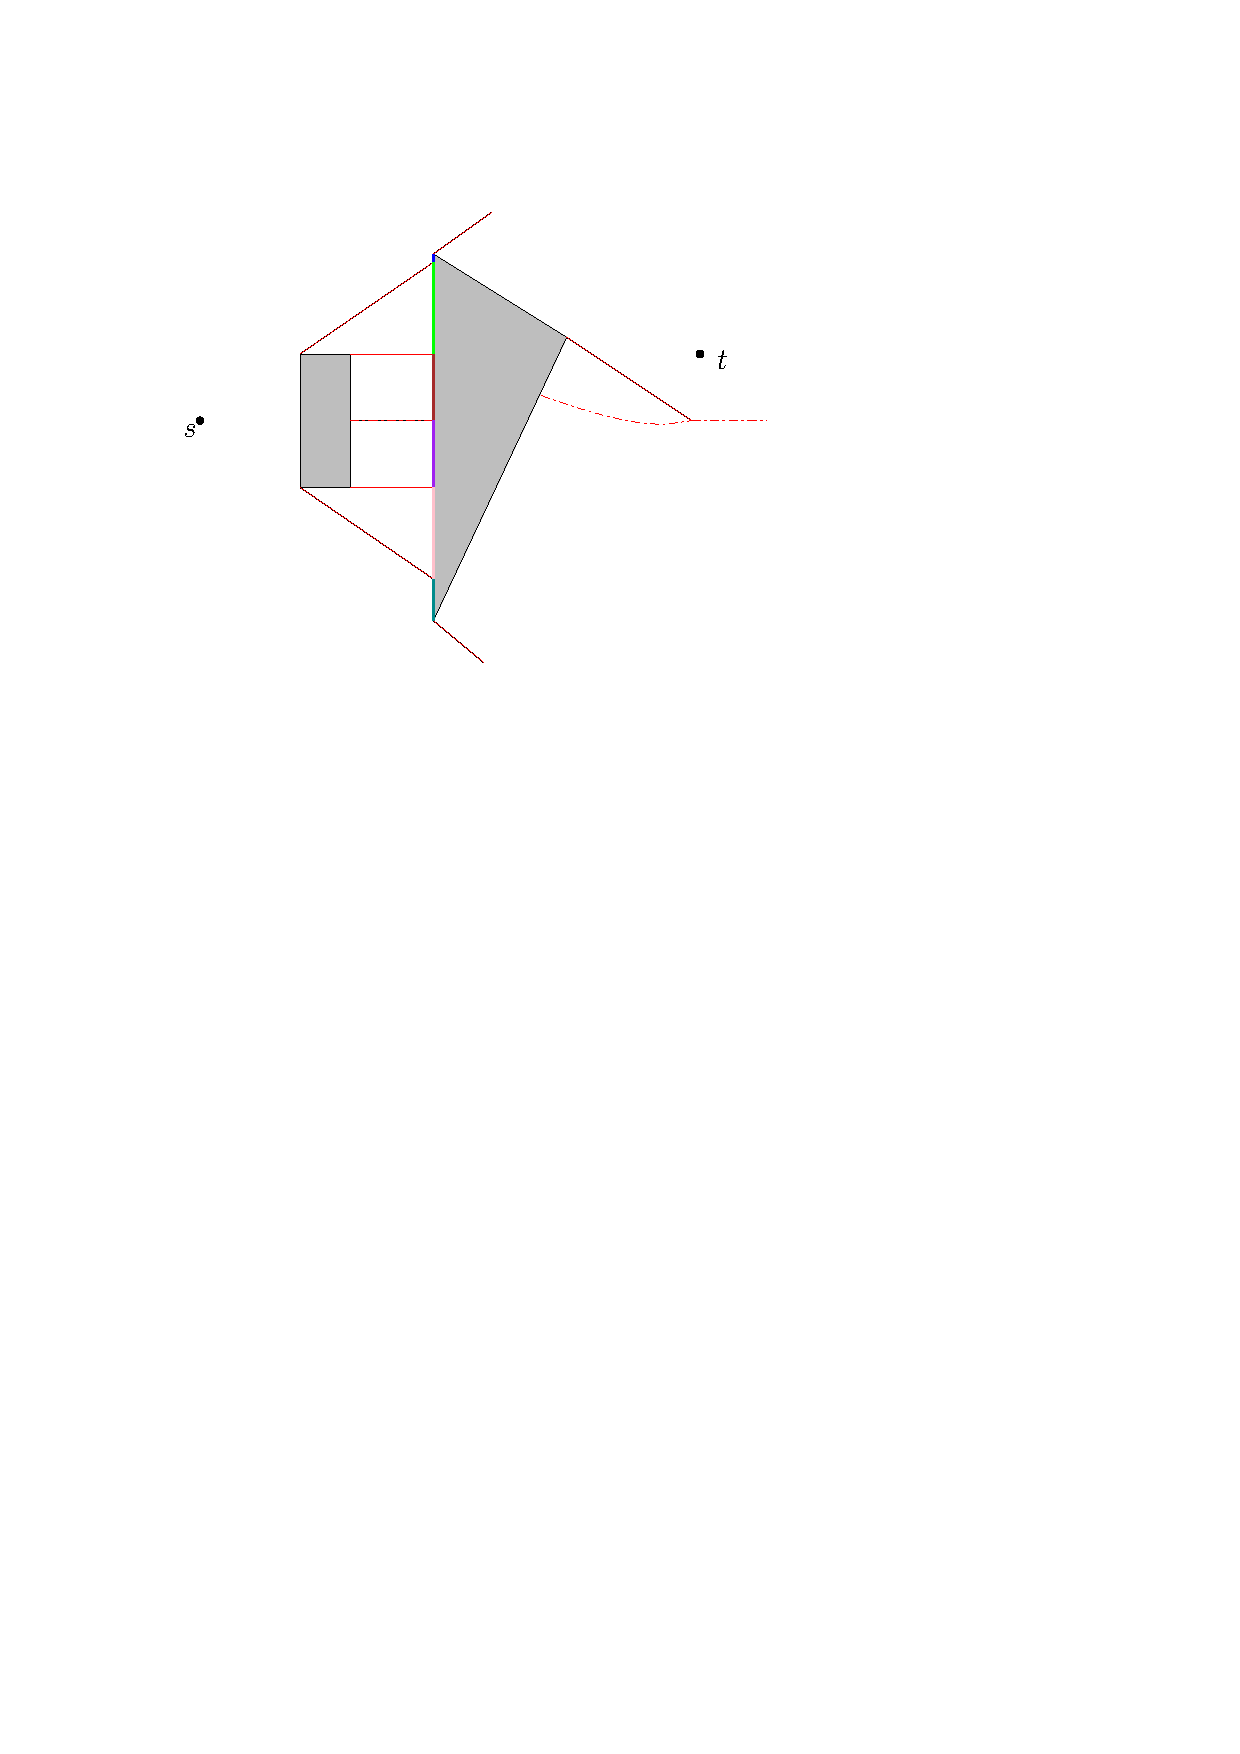
\includegraphics[width=.95\linewidth]{figures/spm0projection.pdf}
  \caption{The preparation of the modified Hershberger-Suri, which will propagate through each 
  		   color on the left most edge of the triangular obstacle}
  \label{fig:spm0projection}
\end{subfigure}%
\begin{subfigure}{.5\textwidth}
  \centering
  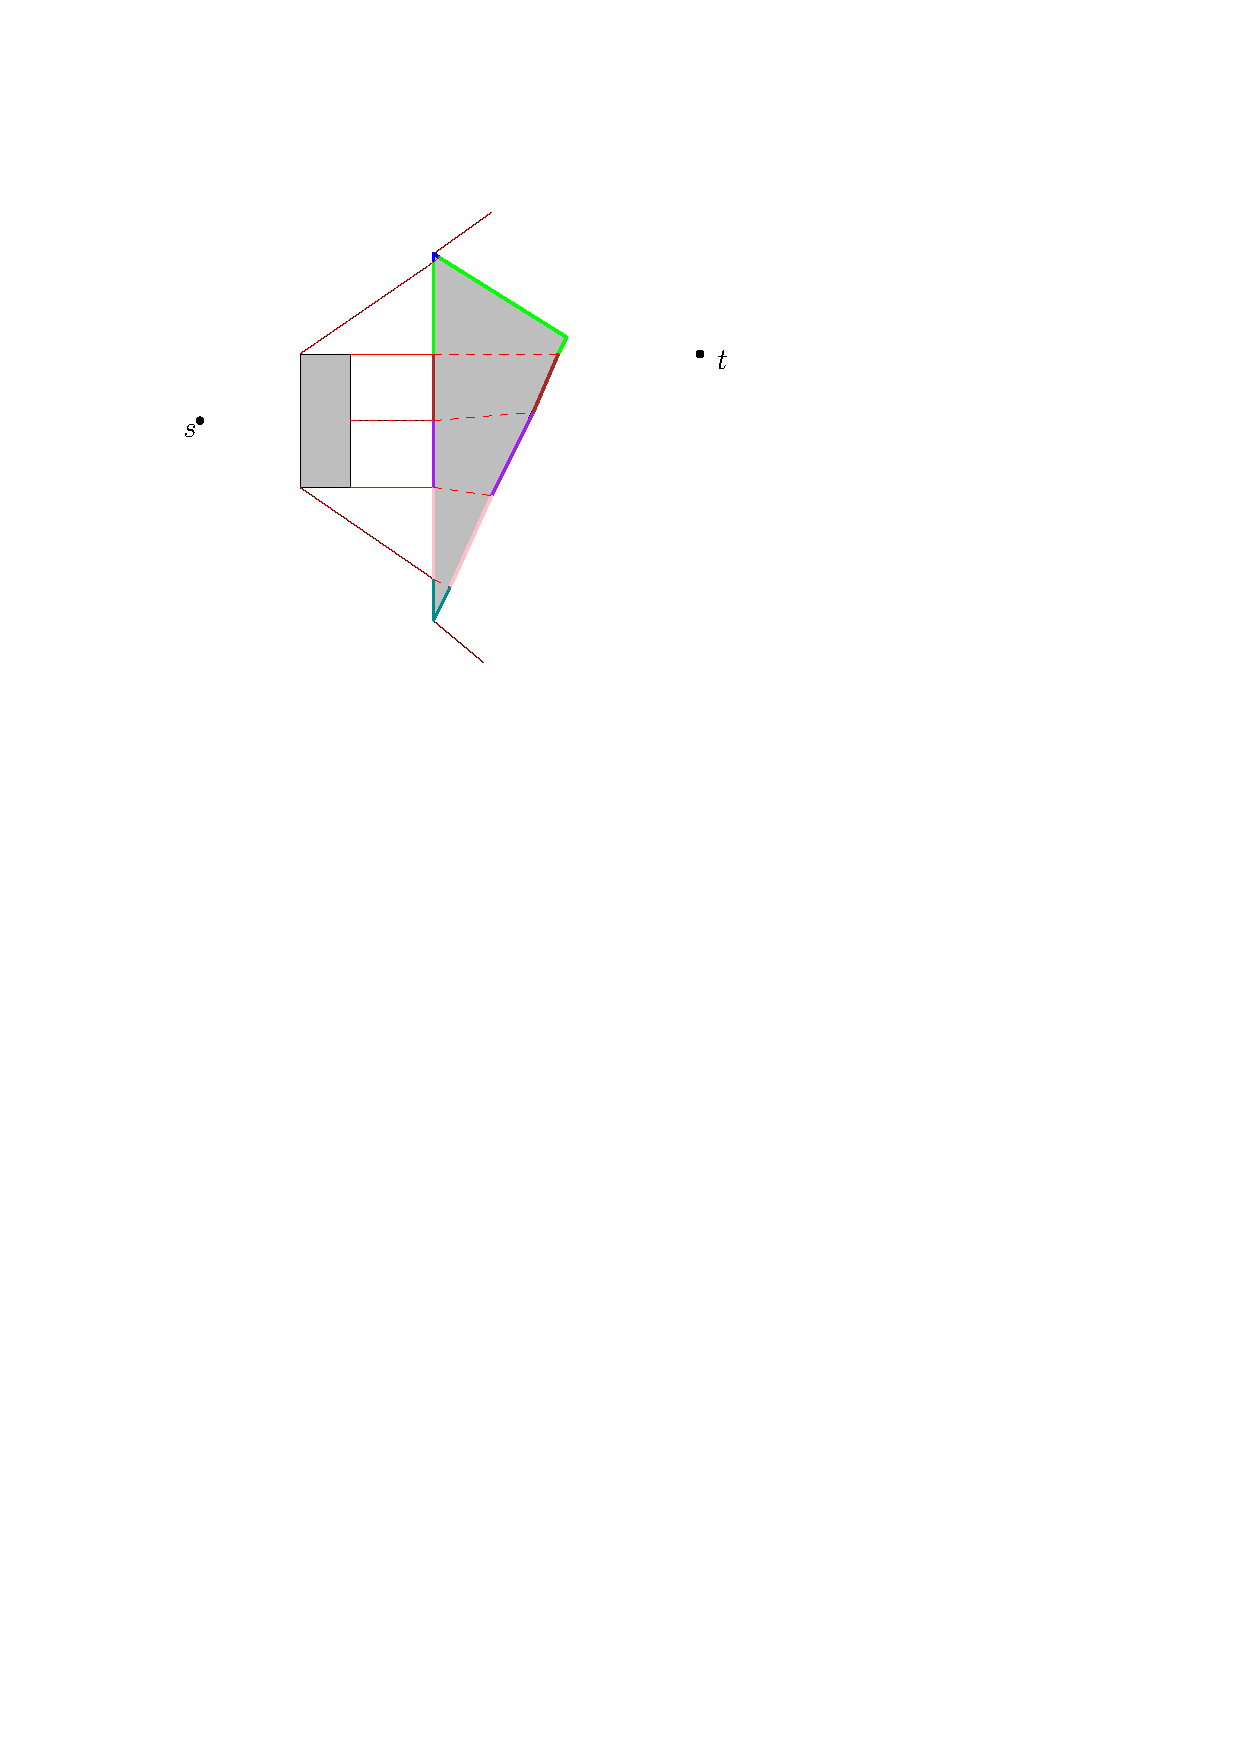
\includegraphics[width=.95\linewidth]{figures/spm1.pdf}
  \caption{the modified Hershberger-Suri algorithm propagates through the triangle to the 
  		   opposite side, where the propagation into the free space will happen for each 
           colored sub-edges as sources}
  \label{fig:spm1}
\end{subfigure}
\end{figure}

The modified algorithm needs to be able to propagate not from a source which is a point but 
from a sub-edge which can be seen in figure \ref{fig:spm0projection}. Each of the colors 
represent a "sub-edge-source" from which wavefronts will propagate the obstacle. When the 
obstacles interior has been propagated, the modified algorithm is ready to propagate the free 
space towards $t$, which we see in figure \ref{fig:spm1}. It's worth noting that the free area 
the modified algorithm needs to propagate in figure \ref{fig:spm1}, is enclosed by the the two 
red line which are collinear with $s$ and the top and bottom point of the triangle, with an 
angle of less than 180 degree. This is due to the area on the other of the wedge could be 
reached faster by just going directly from $s$ without violating an obstacle.

This process is then repeated when constructed the next level of the $SPM_i$ map. Finally we 
will have $SPM_k$ which will consist of an area where the path freely can traverse, since it 
haven't violated more than the allowed obstacles, and a $SPM_{=k}$ which consist of areas, 
where the path needs to make turns since it can't violate any more obstacles. These two areas 
are what $SPM_k$ are made of, and from this we can use the map to look up the fastest path 
from $s$ to $t$.